\documentclass[c, dvipsnames, 8pt]{beamer}  
\usepackage{amsmath}

\usepackage[export]{adjustbox}


\usetheme{Berkeley}

\usefonttheme{professionalfonts} % using non standard fonts for beamer
\usefonttheme{serif} % default family is serif
\usepackage{fontspec}
\setmainfont{Liberation Serif}

\usepackage{unicode-math}      % пакет для установки математического шрифта
\setmathfont{Asana-Math.otf}    % шрифт для математики

\title[OU processes]  
{Ornstein - Uhlenbeck processes. \\  Novikov martingale method.}

%\subtitle{
%}
%

\author[]{Kasianova, Shulyak}
\institute[]{Higher School of Economics}

\date{\today}

\begin{document}
	
	
\maketitle

\section{Some results on AR(1)}

%\subsection{Some results on AR(1)}


\begin{frame}[shrink=5]


\frametitle{\insertsection} 
\begin{figure}
	\centering
	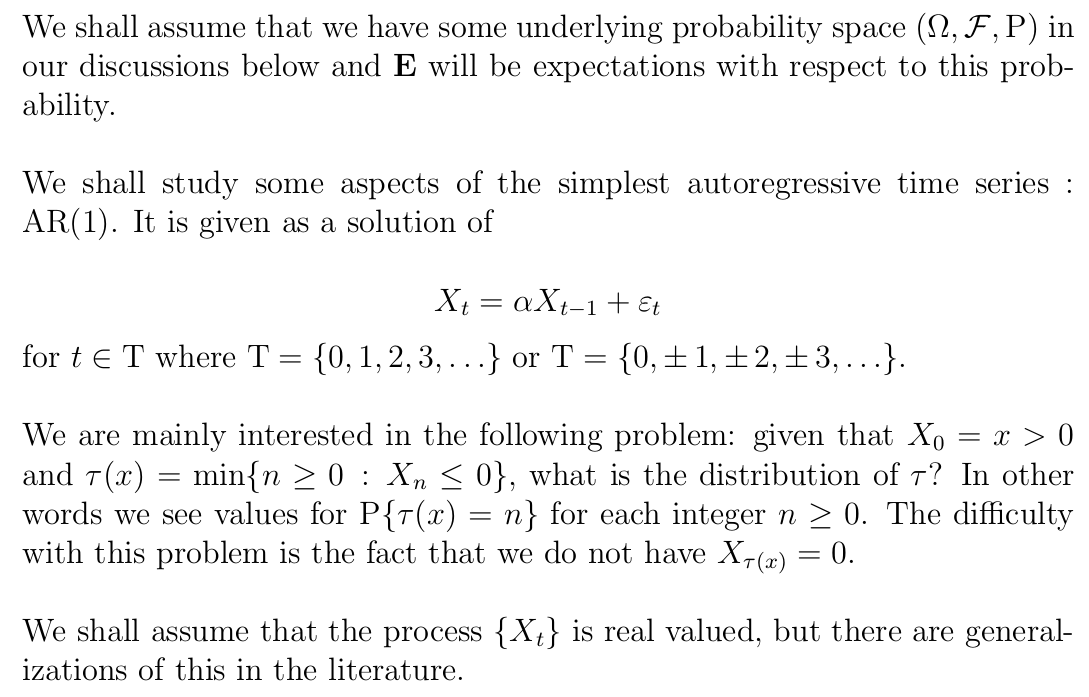
\includegraphics[width=1\linewidth]{screenshot002}
%	\caption{}
	\label{fig:screenshot001}
\end{figure}


%\framesubtitle{\insertsubsection} 


%\begin{block}{Definition 4.4.1}
%	 123
%\end{block}

\end{frame}




\begin{frame}[shrink=5]


\frametitle{\insertsection} 
\begin{figure}
	\centering
	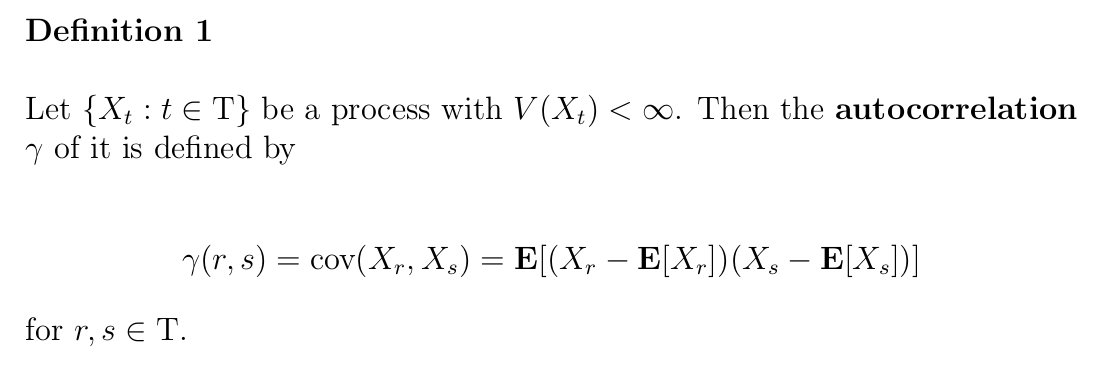
\includegraphics[width=1\linewidth]{screenshot003}
	%	\caption{}
	\label{fig:screenshot001}
\end{figure}


%\framesubtitle{\insertsubsection} 


%\begin{block}{Definition 4.4.1}
%	 123
%\end{block}

\end{frame}



\begin{frame}[shrink=5]


\frametitle{\insertsection} 
\begin{figure}
	\centering
	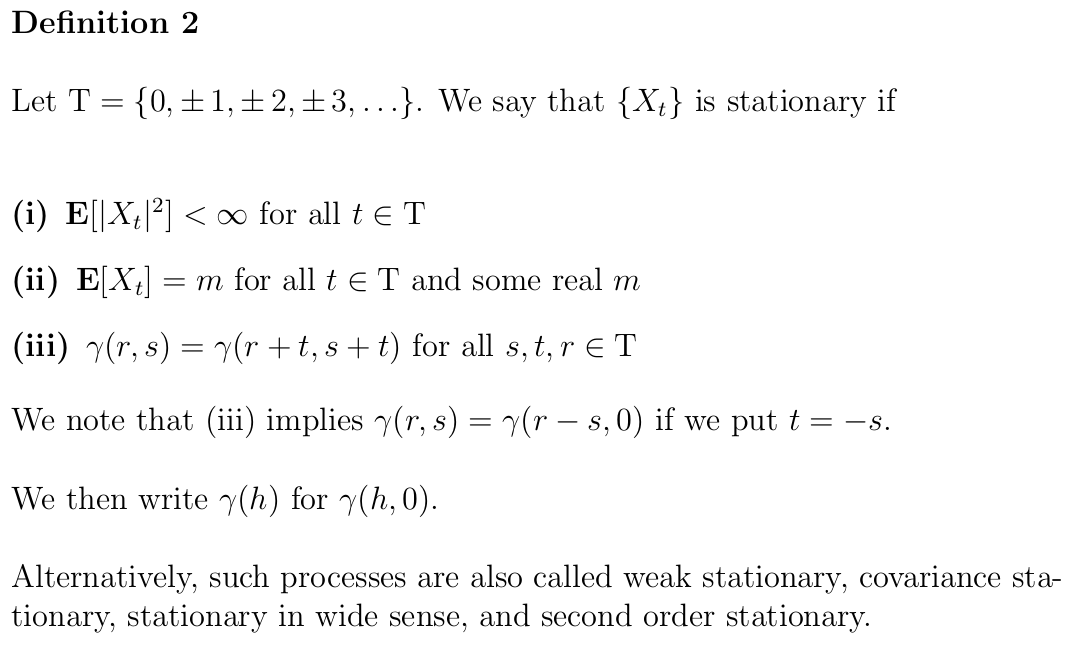
\includegraphics[width=1\linewidth]{screenshot004}
	%	\caption{}
	\label{fig:screenshot001}
\end{figure}

\begin{figure}
%	\left
	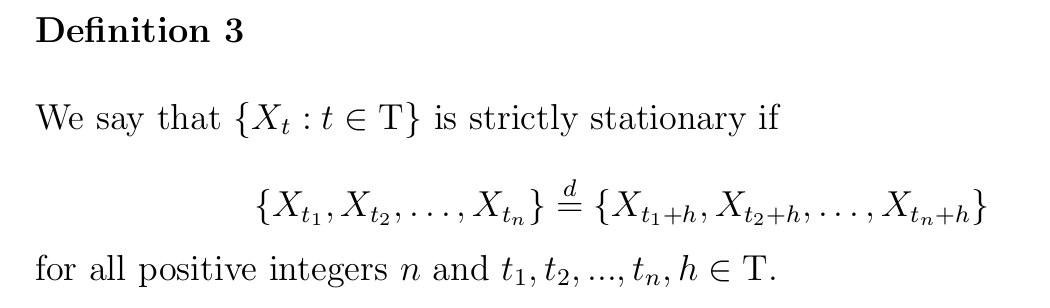
\includegraphics[width=0.9\linewidth,left]{screenshot006}
	%	\caption{}
	\label{fig:screenshot001}
\end{figure}

%\framesubtitle{\insertsubsection} 


%\begin{block}{Definition 4.4.1}
%	 123
%\end{block}

\end{frame}



\begin{frame}[shrink=5]


\frametitle{\insertsection} 
\begin{figure}
	\centering
	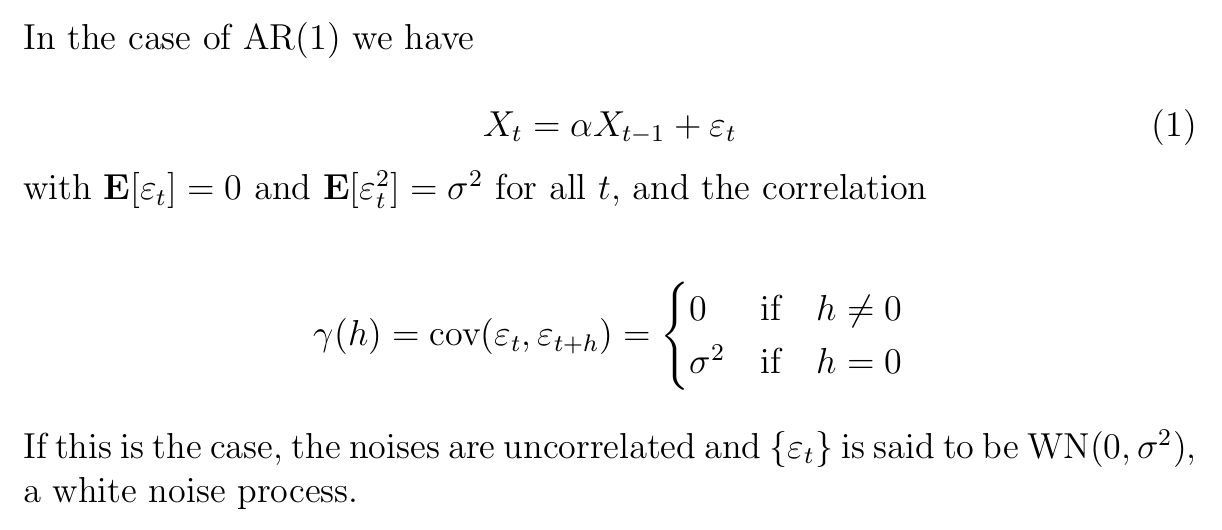
\includegraphics[width=1\linewidth]{screenshot007}
	%	\caption{}
	\label{fig:screenshot001}
\end{figure}

\frametitle{\insertsection} 
\begin{figure}
	\centering
	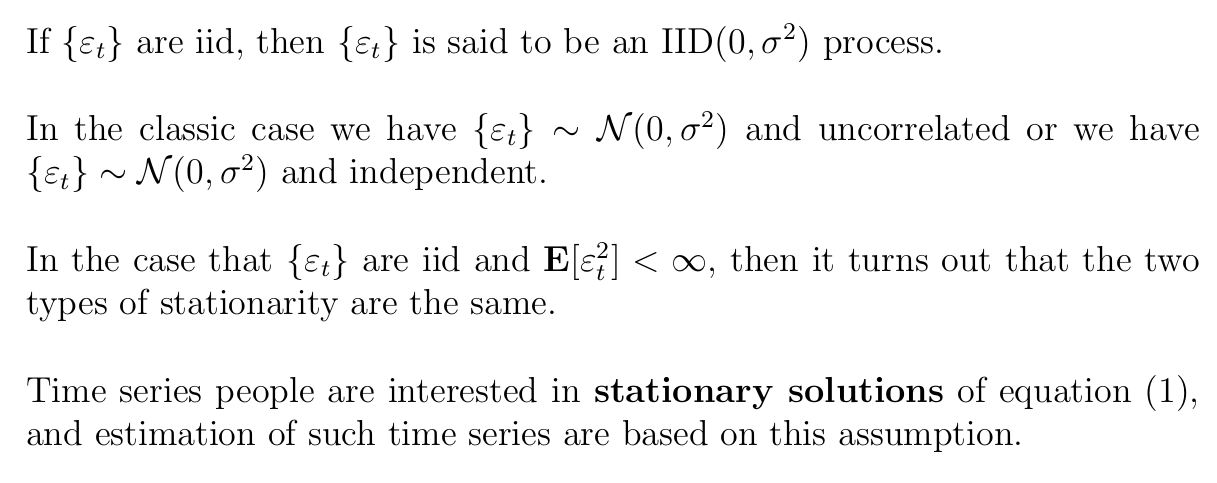
\includegraphics[width=1\linewidth]{screenshot008}
	%	\caption{}
	\label{fig:screenshot001}
\end{figure}





\end{frame}



%
%\section{Example 1}
%
%
%
%
%\begin{frame}[shrink=5]
%	
%	
%	\frametitle{\insertsection} 
%	\begin{figure}
%		\centering
%		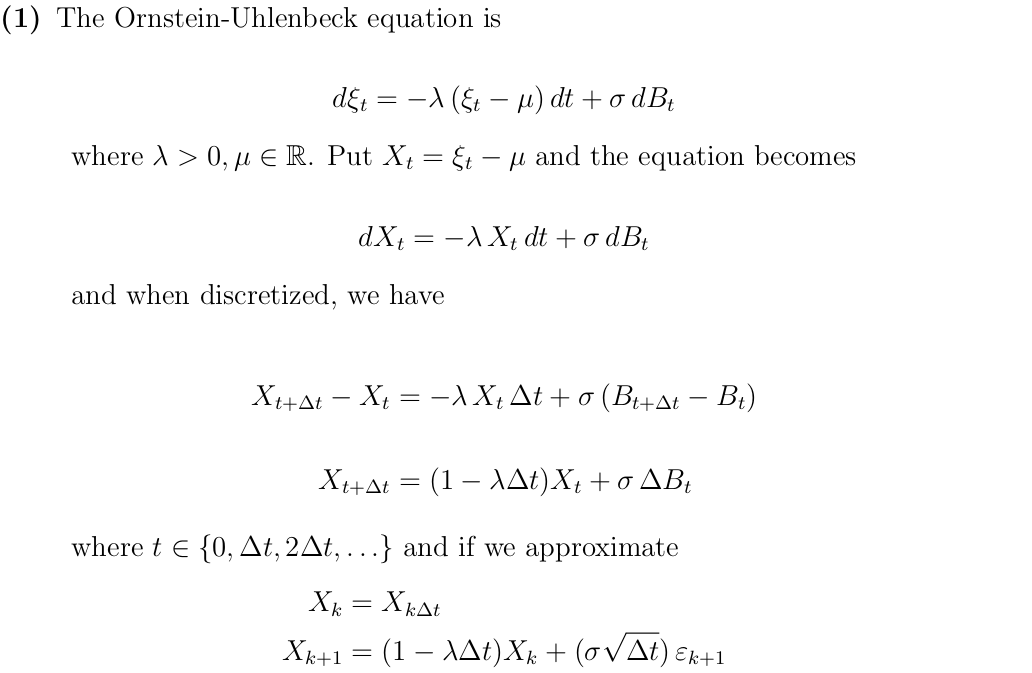
\includegraphics[width=1\linewidth]{screenshot009}
%		%	\caption{}
%		\label{fig:screenshot001}
%	\end{figure}
%
%
%	
%	\frametitle{\insertsection} 
%	\begin{figure}
%		\centering
%		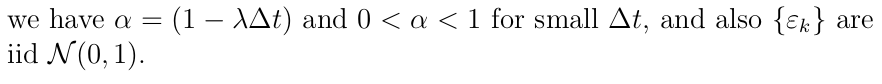
\includegraphics[width=0.8\linewidth, left]{screenshot010}
%		%	\caption{}
%		\label{fig:screenshot001}
%	\end{figure}
%	
%	
%	
%	
%	
%\end{frame}
%
%
%
%\begin{frame}[shrink=5]
%	
%	
%	\frametitle{\insertsection} 
%	\begin{figure}
%		\centering
%		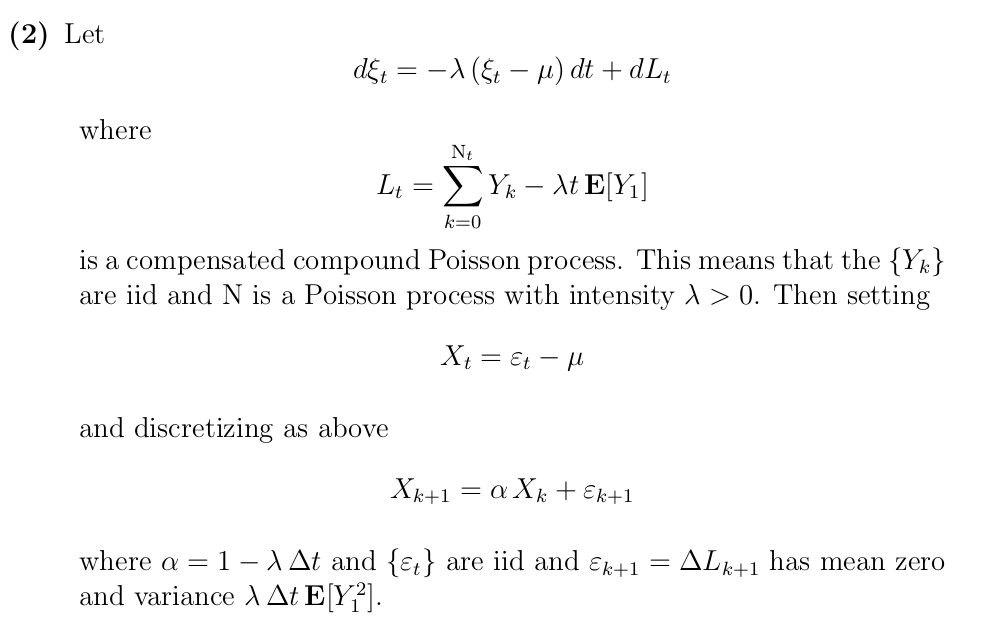
\includegraphics[width=1\linewidth]{screenshot011}
%		%	\caption{}
%		\label{fig:screenshot001}
%	\end{figure}
%	
%	
%	
%	
%\end{frame}


\section{Ornstein - Uhlenbeck processes}




\begin{frame}[shrink=5]
	\frametitle{\insertsection} 
	
	
	Recall 
	
\begin{itemize}
	\item 	Arithmetic BM:  	$dX_t = \mu dt + \sigma d B_t$.
	\item 	Geometric BM:  	$dX_t = \mu X_t dt + \sigma X_t d B_t$.
	\item 	OU process:  	$dX_t = \theta ( \mu  - X_t)  dt + \sigma  d B_t$.
\end{itemize}	


\


OU process is a  mean-reverting process, i.e.  over time, the process tends to drift towards its mean function. 

\

Direction and the magnitude of the drift is not constant but changes depending on the difference between th value of the process and its long term mean.

\

When $X_t$ is below $\mu$ the positive drift pulls it back up towards $\mu$, whereas the opposite occurs when $X_t$ is above $\mu$.  Therefore, 
$\mu$  may be
interpreted as the ``long run mean'' of the process ($E[X_t] \to \mu \ as \  t \to \infty$ )
and the mean-reversion coefficient $\theta$  is the speed of adjustment of $X_t$ towards its long run.
Stochastic term $\sigma d B_t$ captures the instantaneous volatility, i.e. constant instantaneous variance $\sigma^2$, which ensures that the process erratically and continuously fluctuates around the level $\mu$.



%The main features of the process are:
%• the rate
%• a closed form solution for
%$X_t$, for each time $t$, can be negative with positive probability;
%X(t)
%is available, see [23]; it is
%X(t) = X(s)e −θ V as (t−s) +μ V as (1−e −θ V as (t−s) )+σ V as
%Z
%t
%e −θ V as (t−u) dW (u)
%s
%where
%s ≤ t .
%In particular, as in [24],
%X(t)
%is a Gaussian process with mean and variance
%given respectively by
%E[X(t)|X(s)] = μ V as + (X(s) − μ V as )e −θ V as (t−s)
%V ar[X(t)|X(s)] =
%σ V 2 as
%(1 − e −2θ V as (t−s) ).
%2θ V as
%For simulation purpose, we need to discretize the stochastic dierential equa-
%tion (8), which turns out to be the limiting case as
%t i − t i−1 → 0
%of the discrete
%rst order auto-regressive process (see [24])
%X(t i ) = X(t i−1 )e −θ V as (t i −t i−1 ) +
%s
%+ μ V as (1 − e
%−θ V as (t i −t i−1 )
%) + σ V as
%(1 − e −2θ V as (t i −t i−1 )
%N 0,1 .
%2θ V as


\


\end{frame}


\begin{frame}[shrink=5]
	
\begin{equation}\label{key}
		dX_t = \theta ( \mu  - X_t)  dt + \sigma  d B_t
\end{equation}


Figure 1 shows three sample paths of equation (1) for $\sigma = 0.05$, $\mu = 1 $,
and for increasing values of $\theta$. It can be seen that the smaller $\theta$, the more
$X_t$ drifts away from $\mu$. For $\theta = 2$, $X_t$ displays only small and short-lived deviations from $\mu$.


	\frametitle{\insertsection} 
\begin{figure}
	\centering
	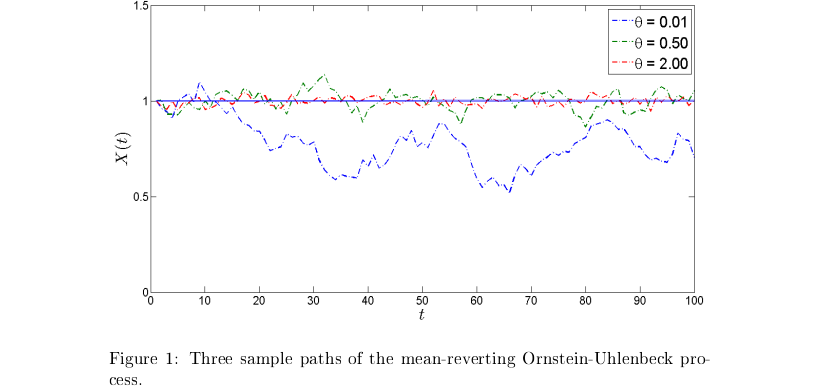
\includegraphics[width=1\linewidth]{screenshot014}
	%	\caption{}
	\label{fig:screenshot001}
\end{figure}


\end{frame}



\begin{frame}[shrink=5]



To solve SDE

\begin{equation}\label{key}
dX_t = \theta ( \mu  - X_t)  dt + \sigma  d B_t
\end{equation}

let's first consider the deterministic version of this equation


\begin{equation}\label{key}
dX_t = \theta ( \mu  - X_t)  dt 
\end{equation}



\begin{equation}\label{key}
dX_t  + \theta  X_t dt = \theta  \mu    dt 
\end{equation}



\begin{equation}\label{key}
\dfrac{dX_t}{dt}  + \theta  X_t = \theta  \mu    
\end{equation}

Can be solved via the integrating factor method.

The integrating factor  is $e^{\int_0^t \theta ds } = e^{\theta t}$ 


\begin{equation}\label{key}
e^{\theta t} \dfrac{dX_t}{dt}  +  e^{\theta t} \theta  X_t = e^{\kappa t}  \theta  \mu    
\end{equation}

The left hand side is an exact differential of the product.

\begin{equation}\label{key}
\dfrac{d}{dt} (e^{\theta t} X_t )    = e^{\theta t}  \theta  \mu    
\end{equation}
	
	
\end{frame}



\begin{frame}[shrink=5]
	
	
	Recall, that for OU process by Ito's lemma $dX_t^2 = \sigma^2 dt  $ 	
	
	\begin{equation}\label{key}
	dX_t = \theta ( \mu  - X_t)  dt + \sigma  d B_t
	\end{equation}
	
	We are looking for solution in a form
	
	
	\begin{equation}\label{key}
	d (e^{\theta t} X_t )    = e^{\theta t}  \theta  \mu   dt 
	\end{equation}
	

	\begin{equation}\label{key}
	dX_t  + \theta  X_t dt = \theta  \mu    dt  + \sigma d B_t
	\end{equation}
	
	Using the same integrating factor
	
	\begin{equation}\label{key}
	e^{\theta t} dX_t  + \theta e^{\theta t}  X_t dt = \theta  \mu e^{\theta t}    dt  + \sigma  e^{\theta t} d B_t
	\end{equation}

	By Ito's product rule $d(e^{\theta t} X_t )  =  d(e^{\theta t}) X_t +   e^{\theta t} d X_t  +  d(e^{\theta t}) d X_t  $,   $d(e^{\theta t}) d X_t  = 0$	as a covariance between a deterministic and stochastic function is zero
	
	
	\begin{equation}\label{key}
	d (e^{\theta t} X_t )    =  \theta  \mu e^{\theta t}    dt  + \sigma  e^{\theta t} d B_t
	\end{equation}
	
	\begin{equation}\label{key}
	\int_0^T d (e^{\theta t} X_t )    = \int_0^T \theta  \mu e^{\theta t}    dt  + \int_0^T \sigma  e^{\theta t} d B_t
	\end{equation}
	
	
	\begin{equation}\label{key}
	e^{\theta T} X_T  -  e^{0} X_0   =  \theta \mu \dfrac{e^{\theta T} - e^{0}  }{\theta}    + \int_0^T \sigma  e^{\theta t} d B_t
	\end{equation}
	
	

	\begin{equation}\label{key}
X_T    =   e^{-\theta T} X_0   +  \mu (1-e^{-\theta T} )     +  \sigma e^{-\theta T} \int_0^T   e^{\theta t} d B_t
\end{equation}
	
\end{frame}




\begin{frame}[shrink=5]
	
SDE: 	
	
	\begin{equation}\label{key}
dX_t = \theta ( \mu  - X_t)  dt + \sigma  d B_t
\end{equation}
	
Solution:
	

\begin{equation}\label{key}
X_T    =   e^{-\theta T} X_0   +  \mu (1-e^{-\theta T} )     +  \sigma \int_0^T   e^{-\theta (T-t)} d B_t
\end{equation}
	
	
	
	

We now characterize its probability distribution. It is easy to see that X is normally distributed, as the integral of a deterministic function w.r.t. Brownian is Gaussian.

The expected value of a deterministic function w.r.t. Brownian is zero. Therefore, 

\begin{equation}\label{key}
E[X_T]    =   E[e^{-\theta T} X_0   +  \mu (1-e^{-\theta T} )     +  \sigma \int_0^T   e^{-\theta (T-t)} d B_t =  e^{-\theta T} X_0   +  \mu (1-e^{-\theta T} )  
\end{equation}

Using Ito's isometry rule 

\begin{equation}\label{key}
E[(\int_0^T X_t dW_t )^2] = E[\int_0^T X^2_t dt]
\end{equation}

gives us a deterministic integral that we can easily evaluate

\begin{equation}\label{key}
Var[X_T]    = E[(X_T-E[X_T] )^2] =   E[ (\sigma \int_0^T   e^{-\theta (T-t)} d B_t)^2] =  \sigma^2 E[  \int_0^T   e^{-2\theta (T-t)} d  t] =   \sigma^2 \dfrac{1 - e^{-2\theta T}}{2\theta}
\end{equation}


\end{frame}



\begin{frame}[shrink=5]

Up to this point we have assumed the start point to be 0 and the end point to be time T. 

The distribution of the value of the process at time T given the information at time 0.

\begin{equation}\label{key}
X_T \sim N(e^{-\theta T} X_0   +  \mu (1-e^{-\theta T} ),  \sigma^2 \dfrac{1 - e^{-2\theta T}}{2\theta} )
\end{equation}
	
We can generalize this to an arbitrary starting point $X_t$


\begin{equation}\label{key}
X_{t+\Delta t } = e^{-\theta \Delta t} X_t   +  \mu (1-e^{-\theta \Delta t} )
 + \sigma \sqrt{\dfrac{1- e^{-2\theta \Delta t}}{2\theta}} N(0,1)
 \end{equation}	

	
It is easy to see that the process is similar to 	AR(1)
	
\begin{equation}\label{key}
y_{t+1} = \beta y_{t} + \alpha + e_{t+1}
\end{equation}	
	
\end{frame}









\begin{frame}[shrink=5]
	
	
	\frametitle{\insertsection} 
	\begin{figure}
		\centering
		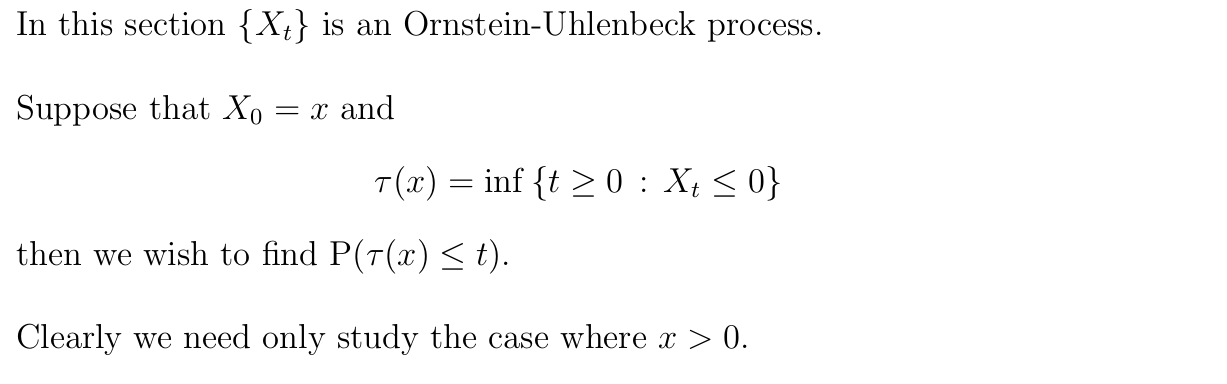
\includegraphics[width=1\linewidth]{screenshot012}
		%	\caption{}
		\label{fig:screenshot001}
	\end{figure}
	

	
\end{frame}





\begin{frame}[shrink=5]
	
	Yi, Chuang. "On the first passage time distribution of an Ornstein–Uhlenbeck process." Quantitative Finance 10, no. 9 (2010): 957-960.
	
	
	
	\
	
	Let 
	\begin{equation}\label{key}
	dX_t = -\alpha X_t dt +\sigma \sqrt{2\alpha} dB_t
	\end{equation}
	
	\frametitle{\insertsection} 
	\begin{figure}
		\centering
		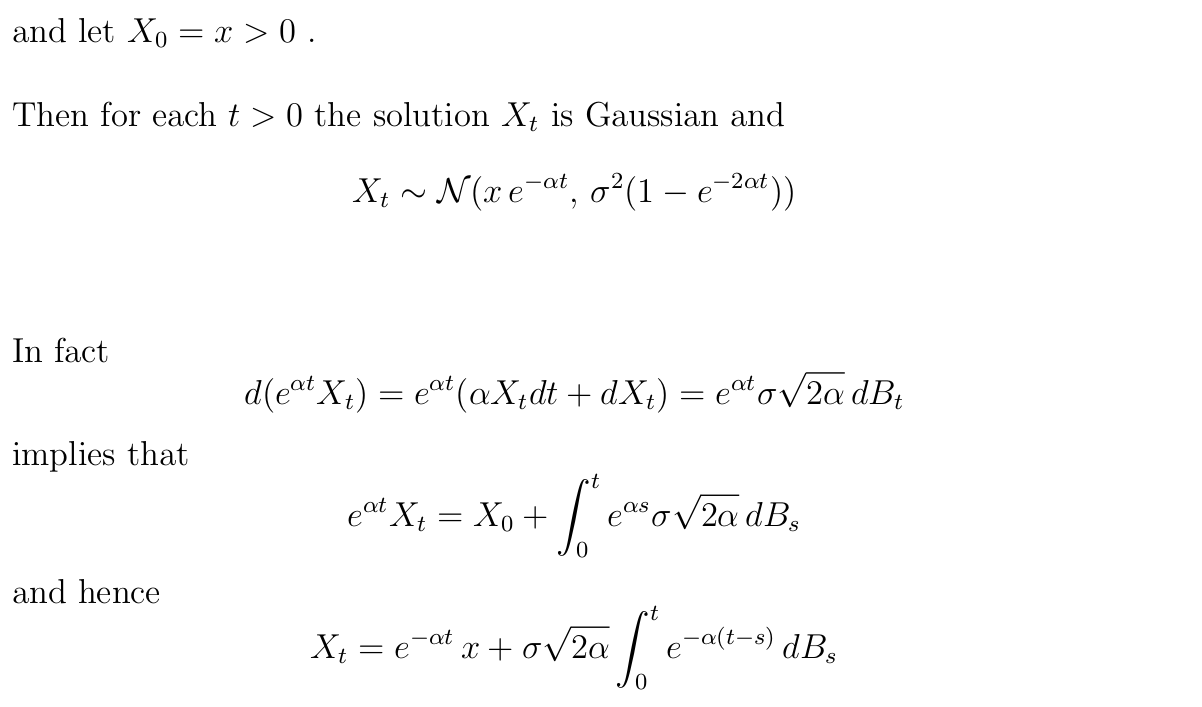
\includegraphics[width=1\linewidth]{screenshot013}
		%	\caption{}
		\label{fig:screenshot001}
	\end{figure}
	
	

	
	
\end{frame}




\begin{frame}[shrink=5]
	
	
	\frametitle{\insertsection} 
	\begin{figure}
		\centering
		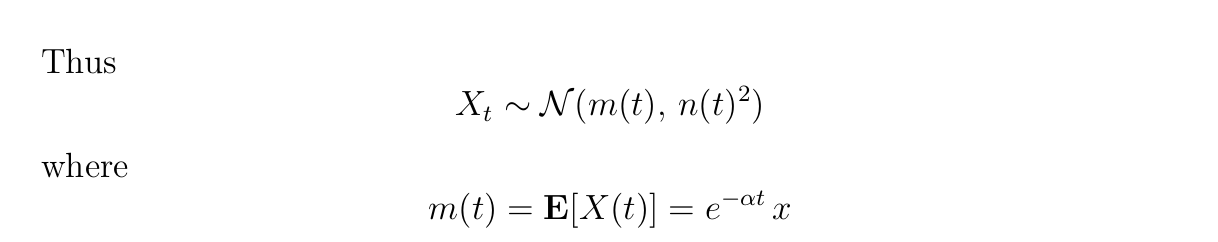
\includegraphics[width=1\linewidth]{screenshot015}
		%	\caption{}
		\label{fig:screenshot001}
	\end{figure}
	
		\frametitle{\insertsection} 
	\begin{figure}
		\centering
		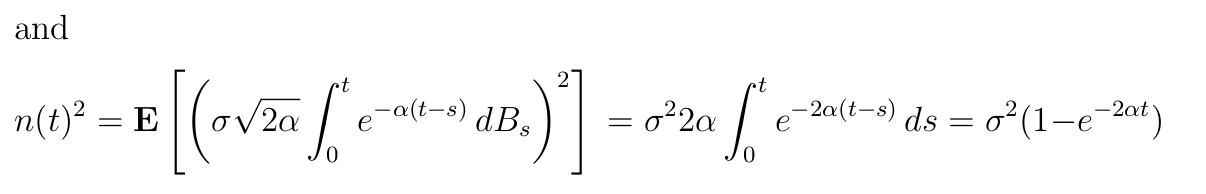
\includegraphics[width=1\linewidth]{screenshot016}
		%	\caption{}
		\label{fig:screenshot001}
	\end{figure}
	
	
		\frametitle{\insertsection} 
	\begin{figure}
		\centering
		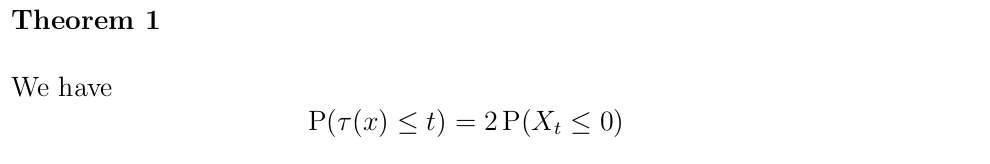
\includegraphics[width=1\linewidth]{screenshot038}
		%	\caption{}
		\label{fig:screenshot001}
	\end{figure}
	
	
	
	
	
	
\end{frame}



\begin{frame}[shrink=5]
	
	
	\frametitle{\insertsection} 
	\begin{figure}
		\centering
		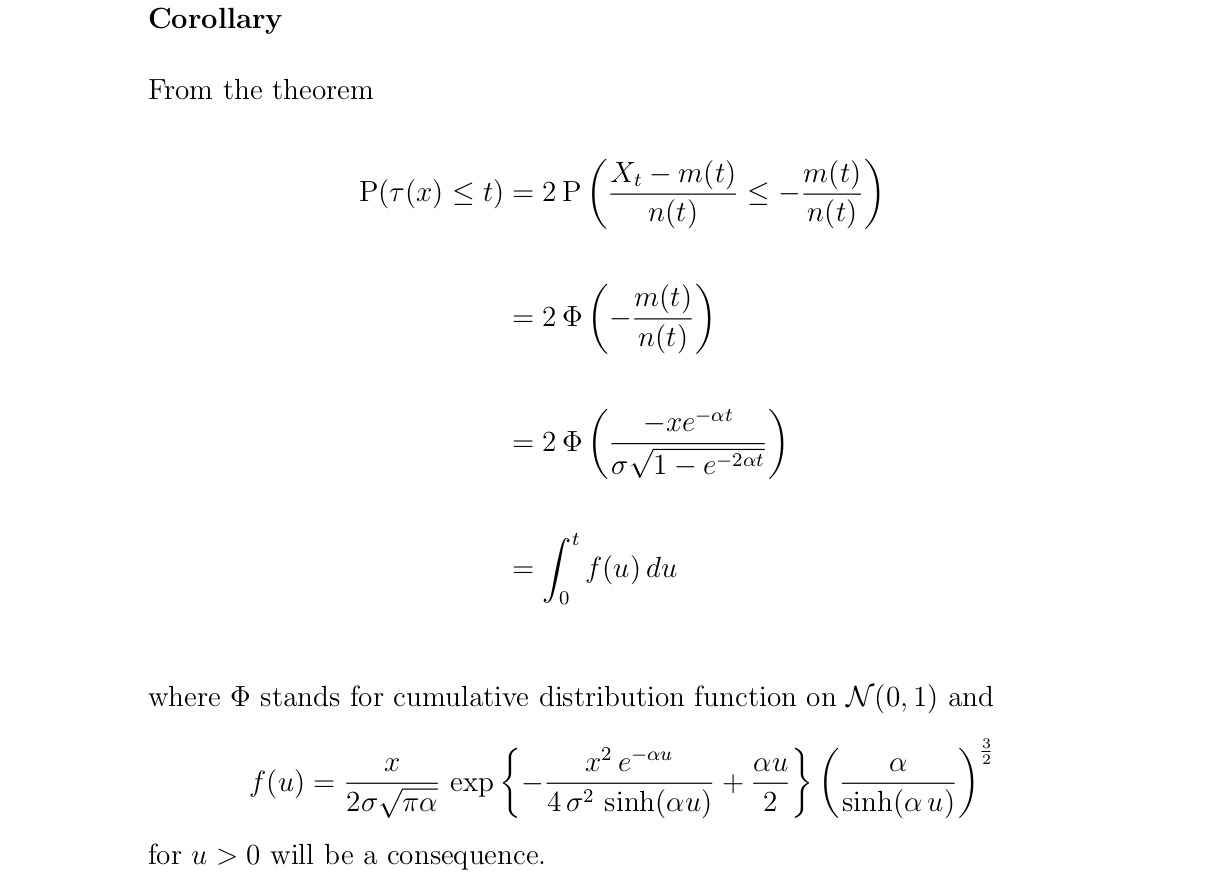
\includegraphics[width=1\linewidth]{screenshot018}
		%	\caption{}
		\label{fig:screenshot001}
	\end{figure}
	


	
	
	
	
	
\end{frame}




\begin{frame}[shrink=5]
	
	
	\frametitle{\insertsection} 
	\begin{figure}
		\centering
		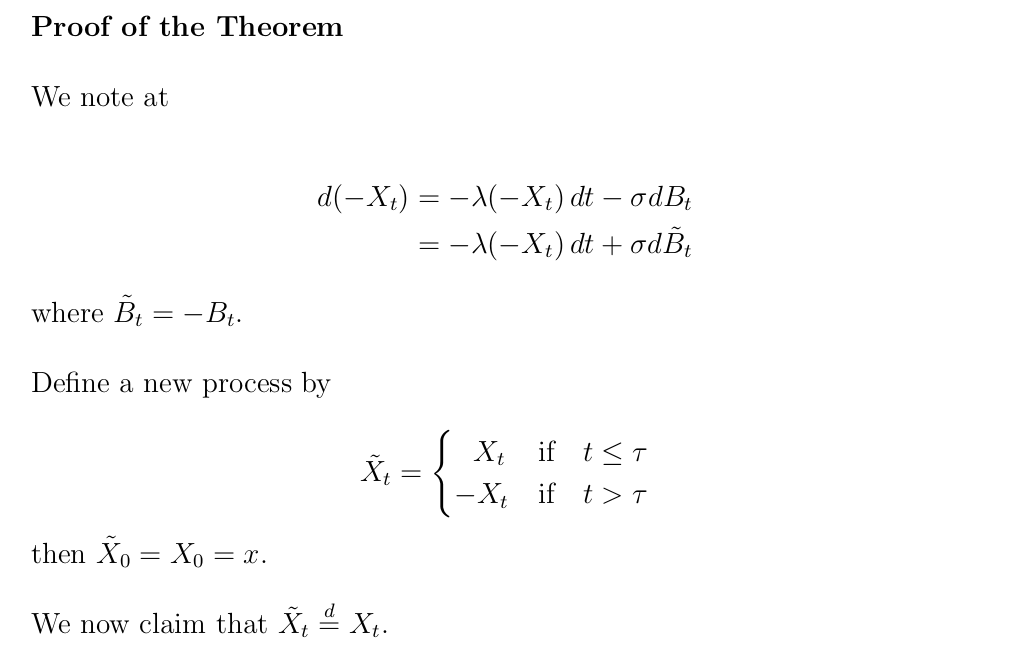
\includegraphics[width=1\linewidth]{screenshot019}
		%	\caption{}
		\label{fig:screenshot001}
	\end{figure}
	
	
	
	
	
	
	
	
\end{frame}


\begin{frame}[shrink=5]
	
	
	\frametitle{\insertsection} 
	\begin{figure}
		\centering
		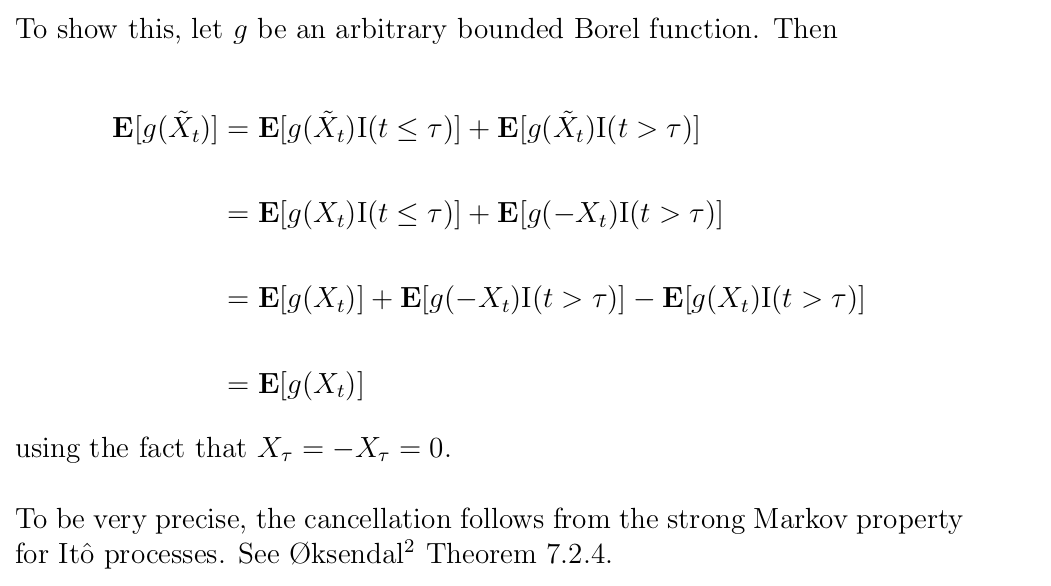
\includegraphics[width=1\linewidth]{screenshot020}
		%	\caption{}
		\label{fig:screenshot001}
	\end{figure}
	
	
	
	
	
	
	
	
\end{frame}




\begin{frame}[shrink=5]
	
	
	\frametitle{\insertsection} 
	\begin{figure}
		\centering
		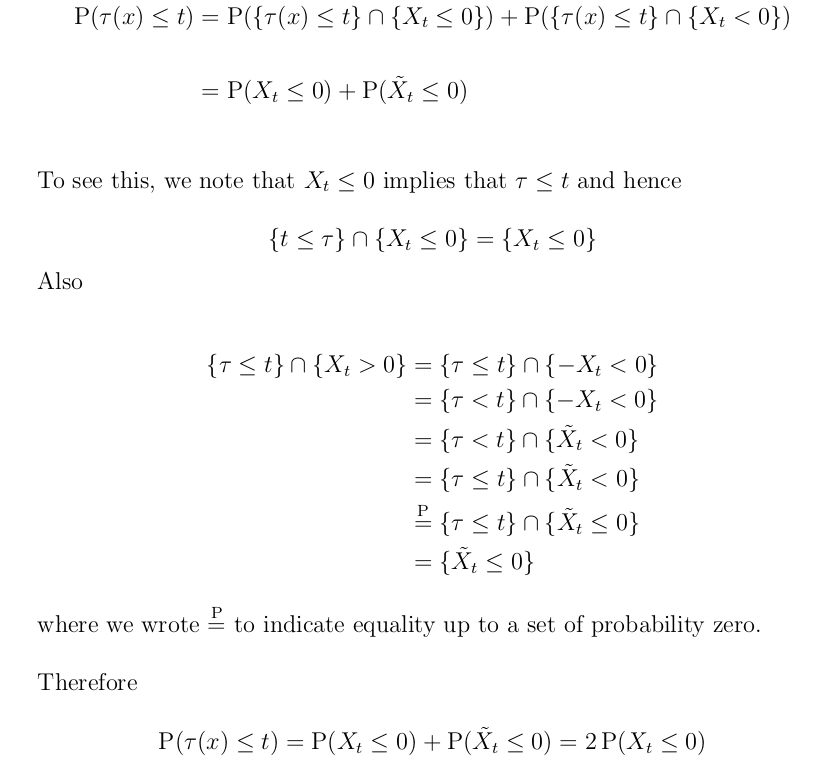
\includegraphics[width=1\linewidth]{screenshot022}
		%	\caption{}
		\label{fig:screenshot001}
	\end{figure}

	
	
	
	
\end{frame}


\section{Stationary Solutions}


\begin{frame}[shrink=5]

	$$X_t = \alpha X_{t-1} + \varepsilon_t   \quad (1)  $$ 
	
	
	\frametitle{\insertsection} 
	\begin{figure}
		\centering
		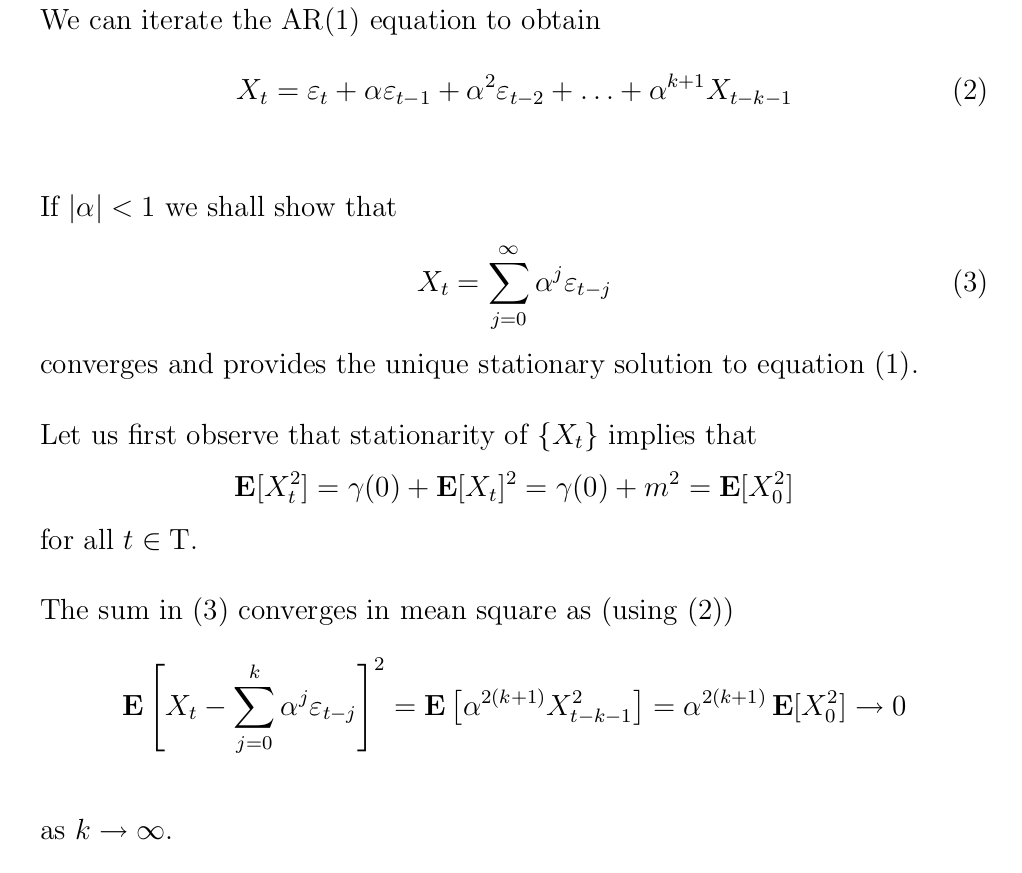
\includegraphics[width=1\linewidth]{screenshot023}
		%	\caption{}
		\label{fig:screenshot001}
	\end{figure}
	
	
\end{frame}





\begin{frame}[shrink=5]
	
From Chebyshev inequality 
	
	\frametitle{\insertsection} 
	\begin{figure}
		\centering
		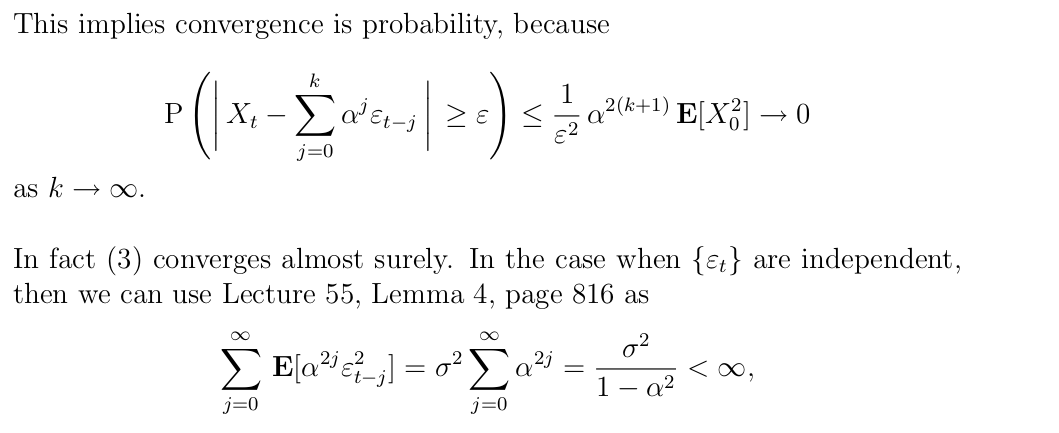
\includegraphics[width=1\linewidth]{screenshot024}
		%	\caption{}
		\label{fig:screenshot001}
	\end{figure}
	
	
\end{frame}






\begin{frame}[shrink=5]
	

	
	\frametitle{\insertsection} 
	\begin{figure}
		\centering
		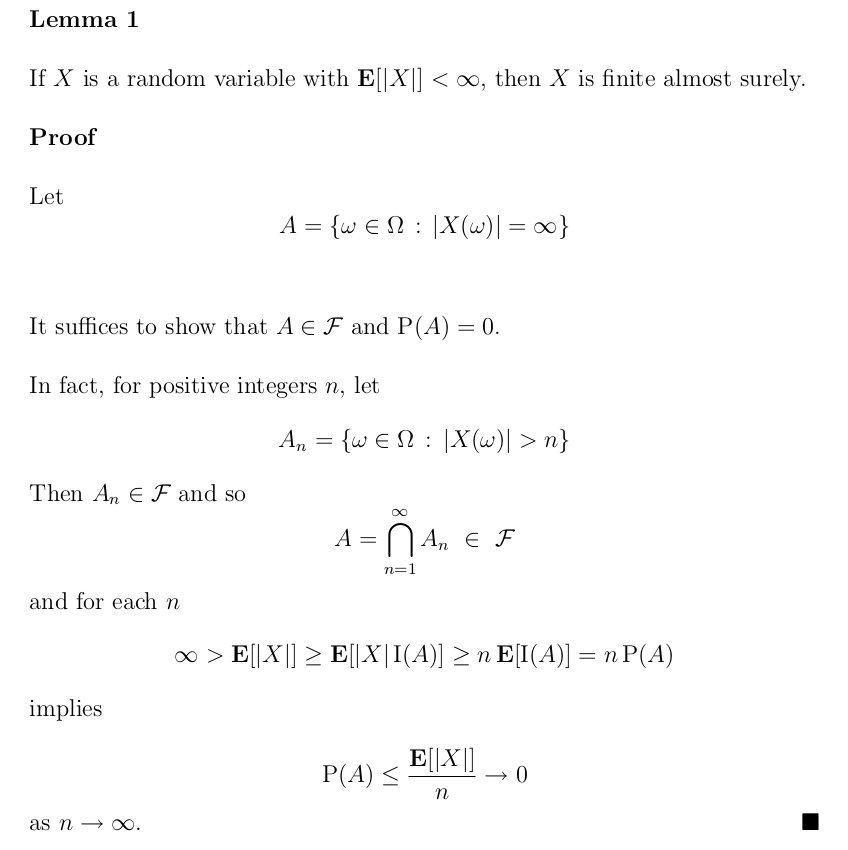
\includegraphics[width=1\linewidth]{screenshot025}
		%	\caption{}
		\label{fig:screenshot001}
	\end{figure}
	
	
\end{frame}



\begin{frame}[shrink=5]
	
	
	
	\frametitle{\insertsection} 
	\begin{figure}
		\centering
		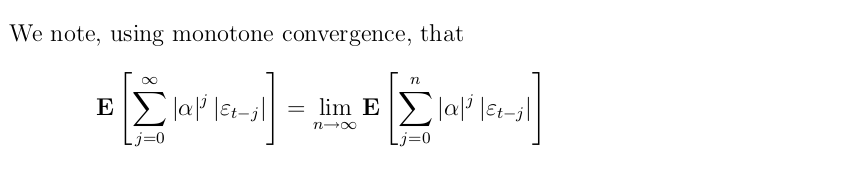
\includegraphics[width=1\linewidth]{screenshot026}
		%	\caption{}
		\label{fig:screenshot001}
	\end{figure}


\frametitle{\insertsection} 
\begin{figure}
	\centering
	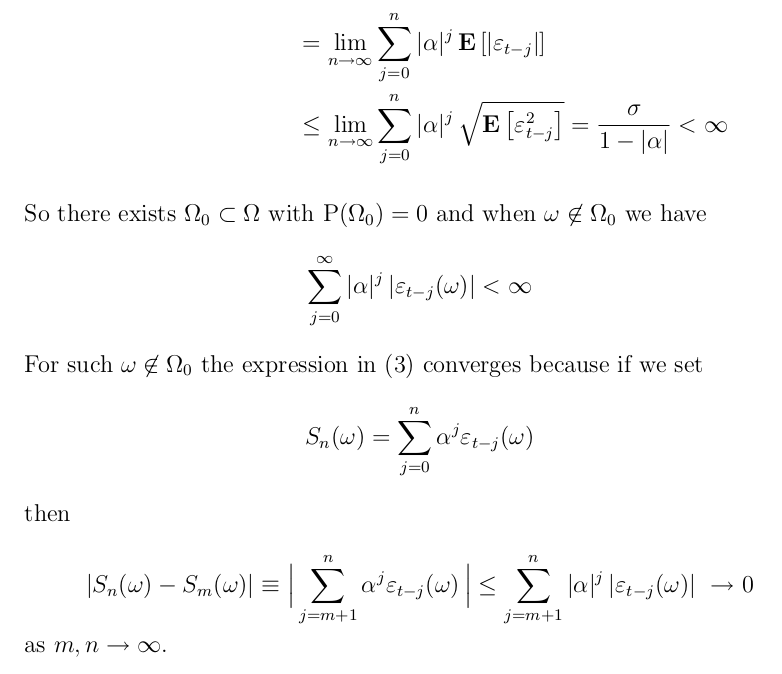
\includegraphics[width=1\linewidth]{screenshot027}
	%	\caption{}
	\label{fig:screenshot001}
\end{figure}
	
	
\end{frame}


\section{Remarks}



\begin{frame}[shrink=5]
	
	
	
	\frametitle{\insertsection} 
	\begin{figure}
		\centering
		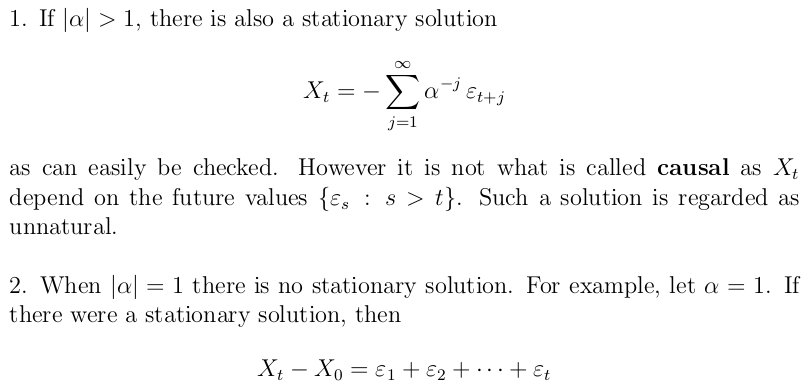
\includegraphics[width=1\linewidth]{screenshot028}
		%	\caption{}
		\label{fig:screenshot001}
	\end{figure}
	
	
	\frametitle{\insertsection} 
	\begin{figure}
		\centering
		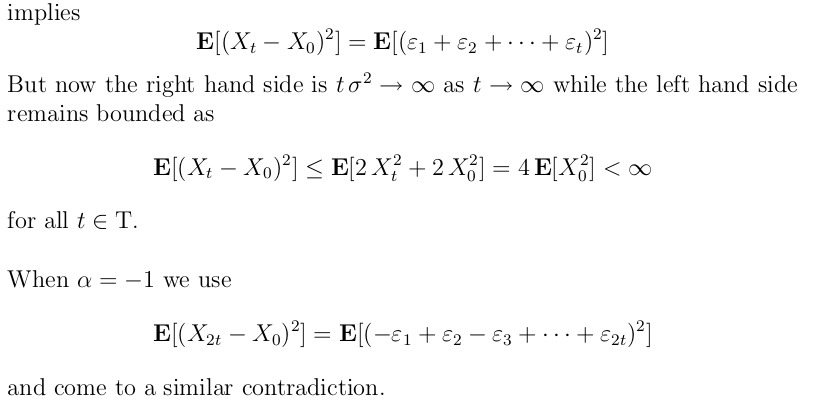
\includegraphics[width=1\linewidth]{screenshot029}
		%	\caption{}
		\label{fig:screenshot001}
	\end{figure}
	
	
\end{frame}





\begin{frame}[shrink=5]
	
	
	
	\frametitle{\insertsection} 
	\begin{figure}
		\centering
		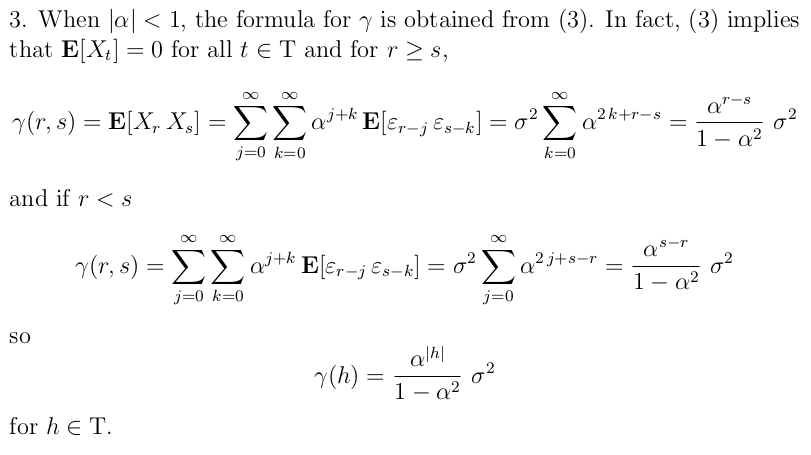
\includegraphics[width=0.7\linewidth]{screenshot030}
		%	\caption{}
		\label{fig:screenshot001}
	\end{figure}
	
		\vfil
	\hfil\hfil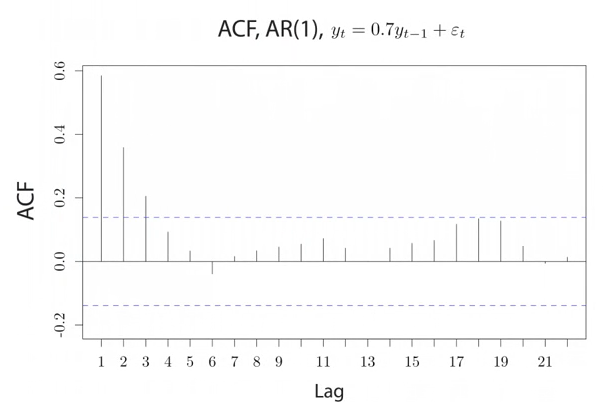
\includegraphics[height=3.5cm]{screenshot031}\hfil\hfil
	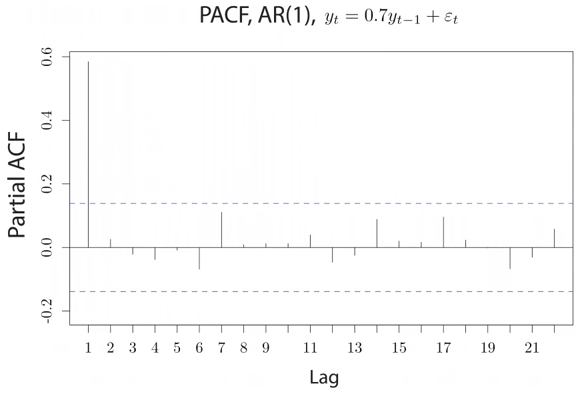
\includegraphics[height=3.5cm]{screenshot032}\newline
	


\end{frame}


\section{Crossing-time problem}


\begin{frame}[shrink=5]
	\frametitle{\insertsection} 
	%\framesubtitle{\insertsubsection} 	
	
	
	\frametitle{\insertsection} 
\begin{figure}
	\centering
	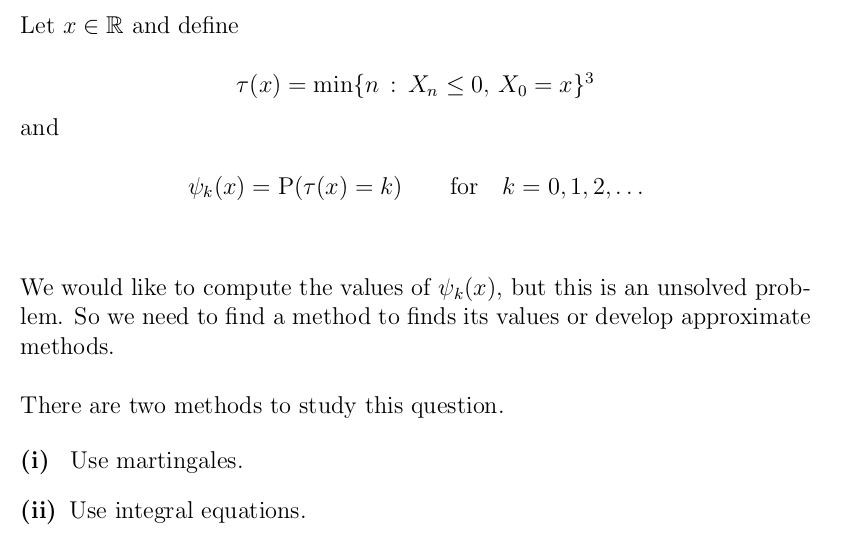
\includegraphics[width=1\linewidth]{screenshot033}
	%	\caption{}
	\label{fig:screenshot001}
\end{figure}

\begin{figure}
	\centering
	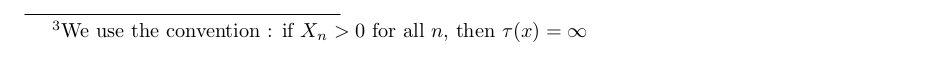
\includegraphics[width=1\linewidth]{screenshot034}
	%	\caption{}
	\label{fig:screenshot001}
\end{figure}




\end{frame}


\section{Integral Equation Methods}

\begin{frame}[shrink=5]
	\frametitle{\insertsection} 


	\begin{figure}
		\centering
		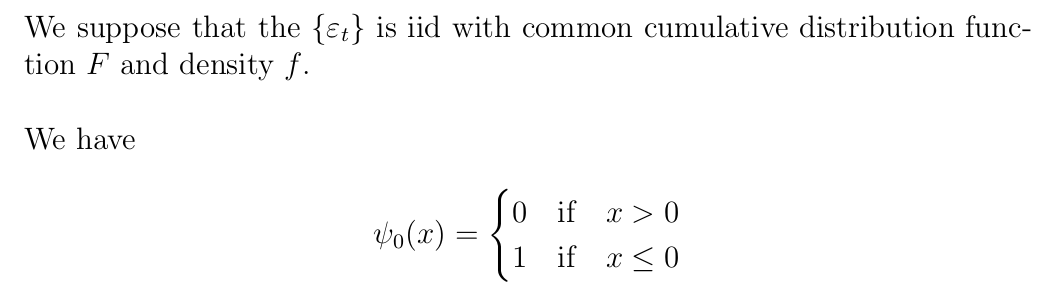
\includegraphics[width=1\linewidth]{screenshot035}
		%	\caption{}
		\label{fig:screenshot001}
	\end{figure}
	
	\begin{figure}
		\centering
		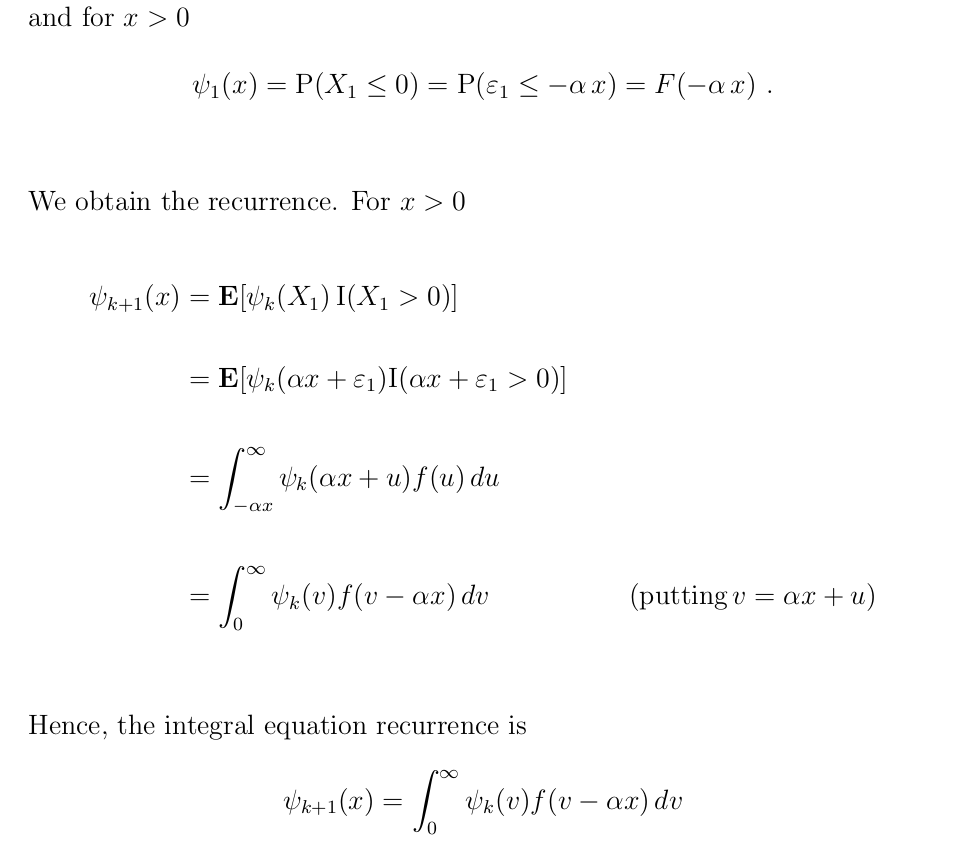
\includegraphics[width=1\linewidth]{screenshot039}
		%	\caption{}
		\label{fig:screenshot001}
	\end{figure}





\end{frame}




\begin{frame}[shrink=5]
	
	
	
	\frametitle{\insertsection} 
	\begin{figure}
		\centering
		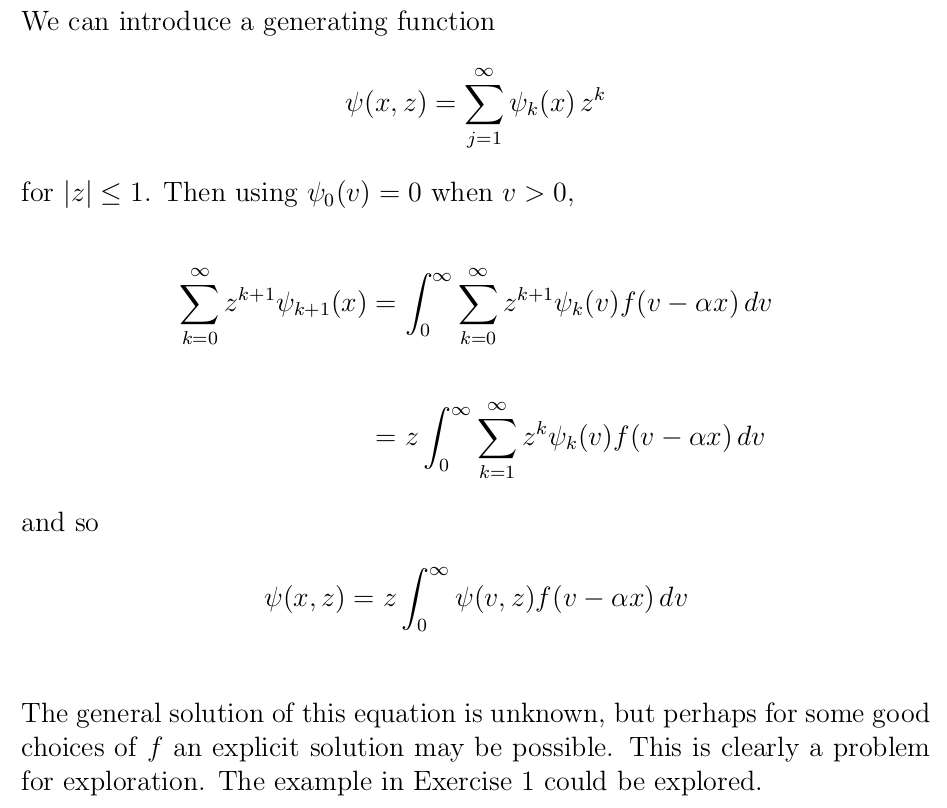
\includegraphics[width=1\linewidth]{screenshot040}
		%	\caption{}
		\label{fig:screenshot001}
	\end{figure}
	
	
	
\end{frame}


%\section{Fortet’s Lemma}
%
%
%\begin{frame}[shrink=5]
%	
%	
%	\frametitle{\insertsection} 
%	\begin{figure}
%		\centering
%		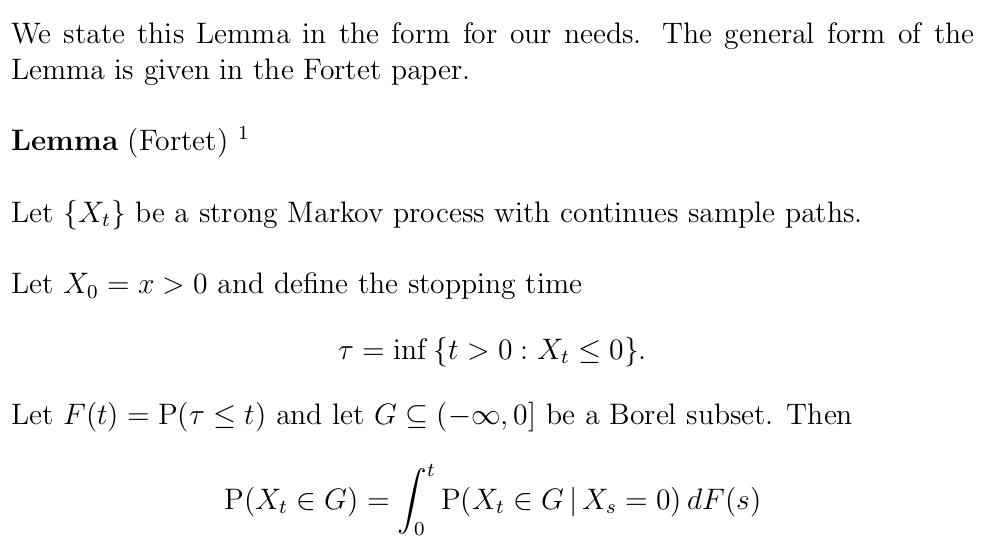
\includegraphics[width=1\linewidth]{screenshot049}
%		%	\caption{}
%		\label{fig:screenshot001}
%	\end{figure}
%	
%	
%\end{frame}



\section{Martingales and first passage times of AR(1) sequences}




\begin{frame}[shrink=5]
	
	
	
	\frametitle{\insertsection} 
	\begin{figure}
		\centering
		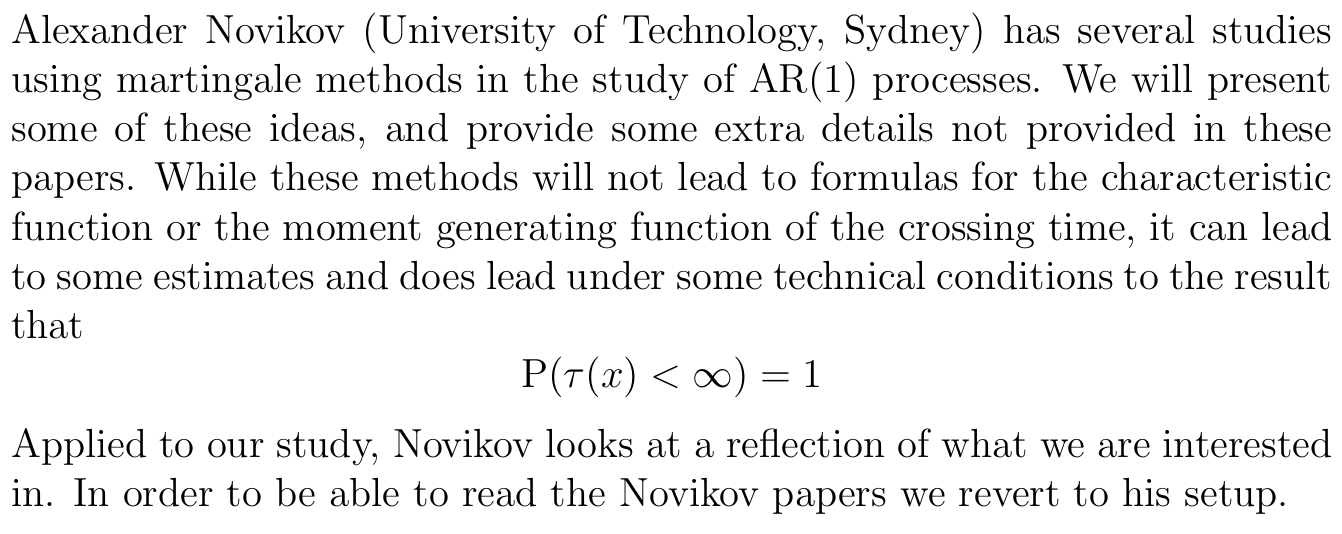
\includegraphics[width=1\linewidth]{screenshot041}
		%	\caption{}
		\label{fig:screenshot001}
	\end{figure}
	
	
\textit{	Abstract}
	
	\
	
	Using the martingale approach we find sufficient conditions for exponential
	boundedness of first passage times over a level for ergodic first order autoregressive
	sequences. Further, we prove a martingale identity to be used in obtaining explicit
	bounds for the expectation of first passage times.
	
	
	\
	
	In applications, the distribution and expectation of such passage times are usually
	approximated via Monte-Carlo simulation or using Markov chain approximations
	(e.g. [16]). However, analytical bounds are also of interest (e.g. to control an accuracy of
	simulation algorithms).
	
\end{frame}


\begin{frame}[shrink=5]
	
	
	
	\frametitle{\insertsection} 
	\begin{figure}
		\centering
		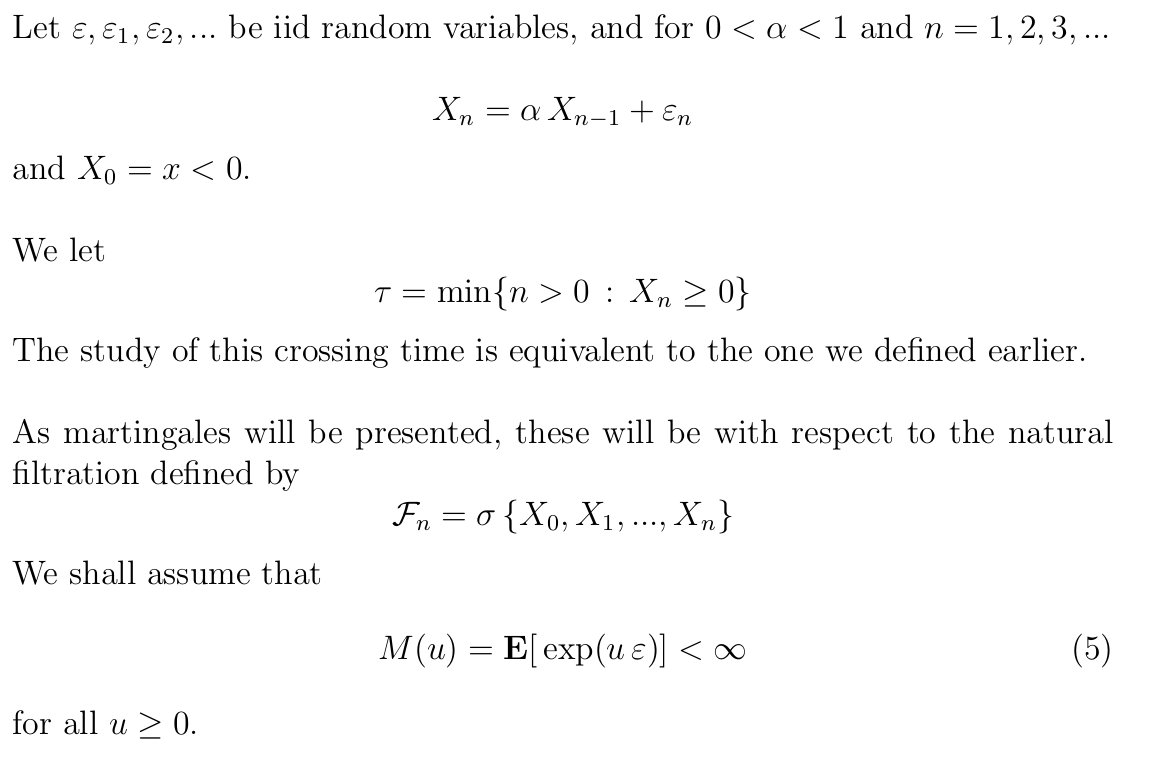
\includegraphics[width=1\linewidth]{screenshot042}
		%	\caption{}
		\label{fig:screenshot001}
	\end{figure}
	
	
	
	
	
\end{frame}





\begin{frame}[shrink=5]
	
	
	
	\frametitle{\insertsection} 
	\begin{figure}
		\centering
		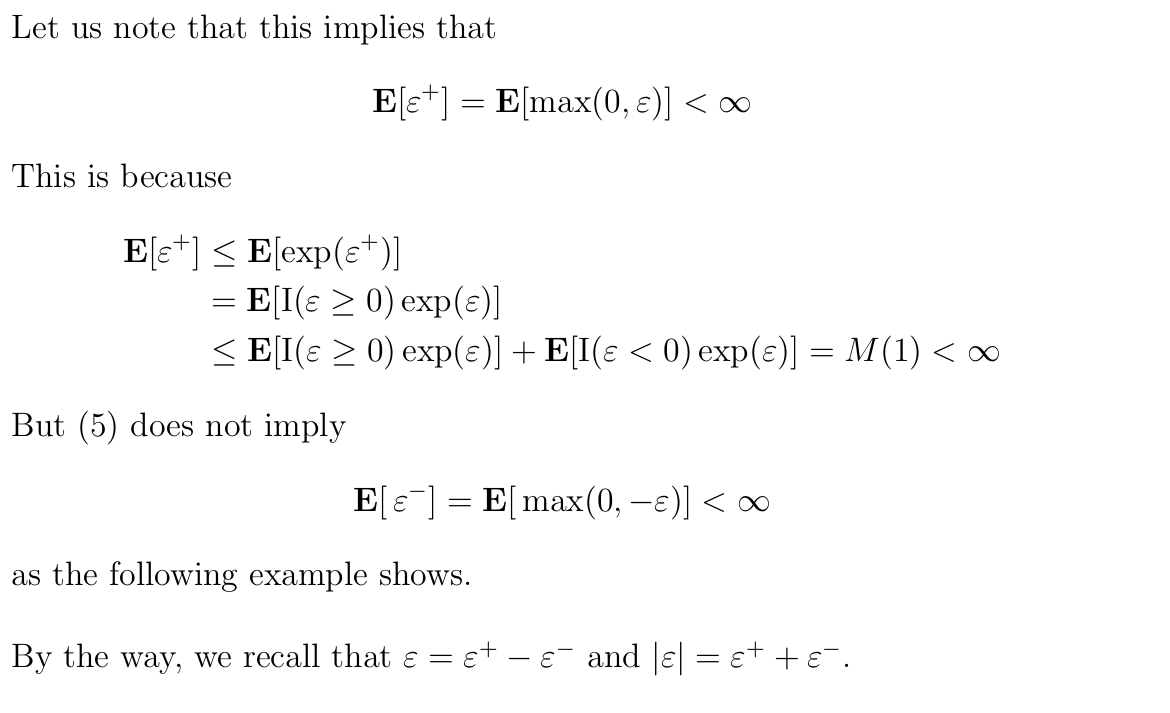
\includegraphics[width=1\linewidth]{screenshot043}
		%	\caption{}
		\label{fig:screenshot001}
	\end{figure}
	
	
	
	
	
\end{frame}


\begin{frame}[shrink=5]
	
	
	\frametitle{\insertsection} 
	\begin{figure}
		\centering
		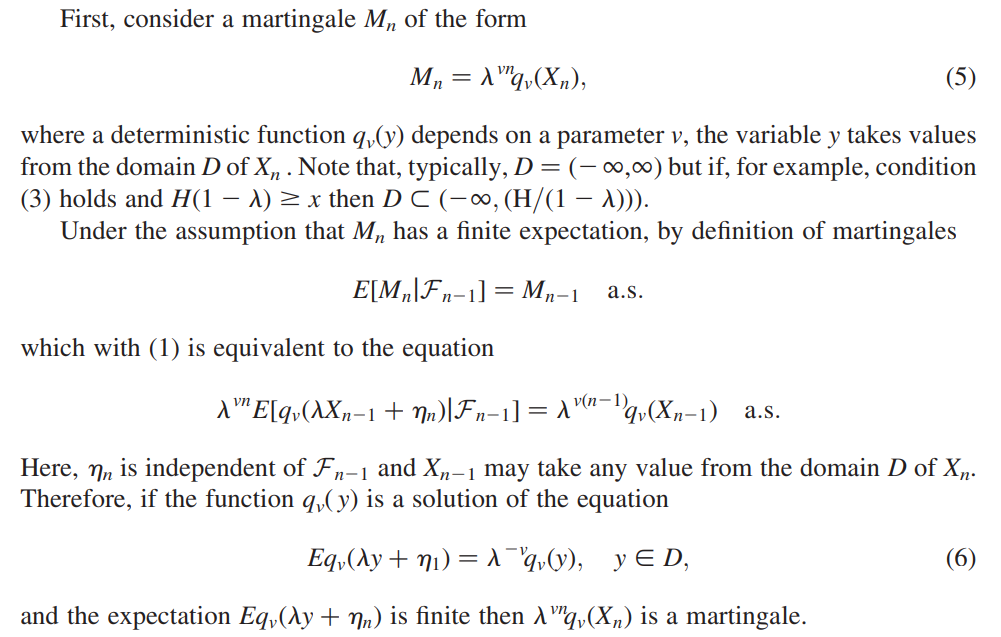
\includegraphics[width=1\linewidth]{screenshot058}
		%	\caption{}
		\label{fig:screenshot001}
	\end{figure}
	
	
	
	
	
	
	
\end{frame}




\section{Vervaat’s Theorem}


\begin{frame}[shrink=5]
	
	
	\frametitle{\insertsection} 
	\begin{figure}
		\centering
		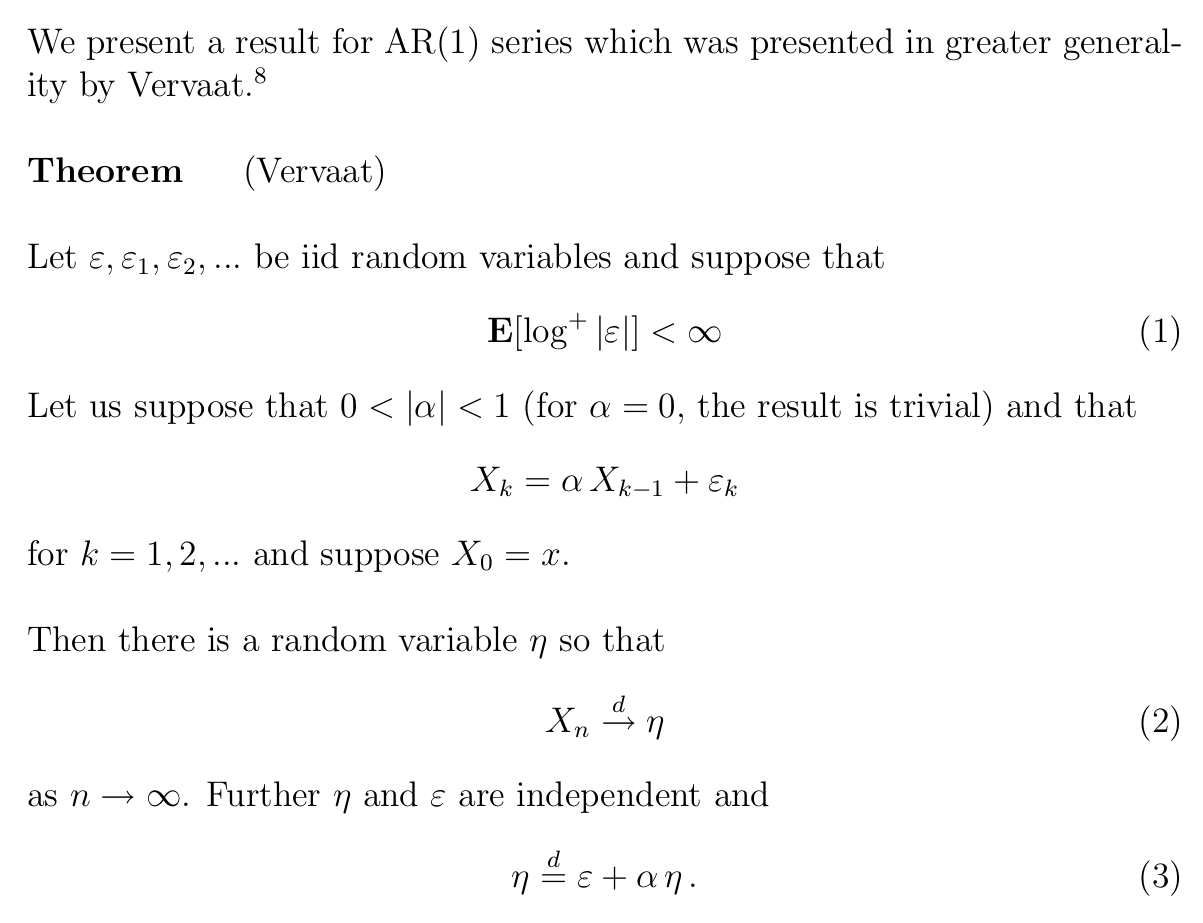
\includegraphics[width=1\linewidth]{screenshot050}
		%	\caption{}
		\label{fig:screenshot001}
	\end{figure}




	
	
\end{frame}



\begin{frame}[shrink=5]
	
	
	\frametitle{\insertsection} 
	\begin{figure}
		\centering
		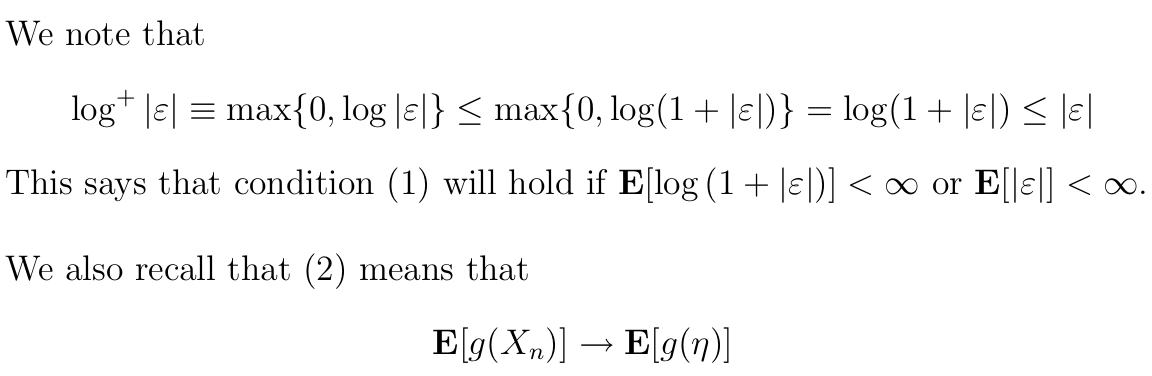
\includegraphics[width=1\linewidth]{screenshot051}
		%	\caption{}
		\label{fig:screenshot001}
	\end{figure}
	
		\frametitle{\insertsection} 
	\begin{figure}
		\centering
		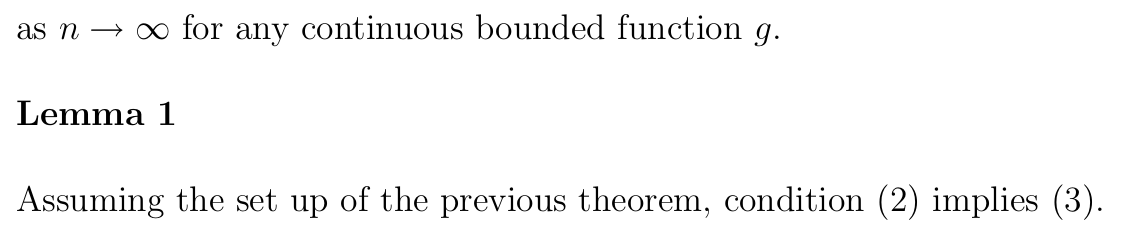
\includegraphics[width=1\linewidth]{screenshot052}
		%	\caption{}
		\label{fig:screenshot001}
	\end{figure}
	
	
			\frametitle{\insertsection} 
	\begin{figure}
		\centering
		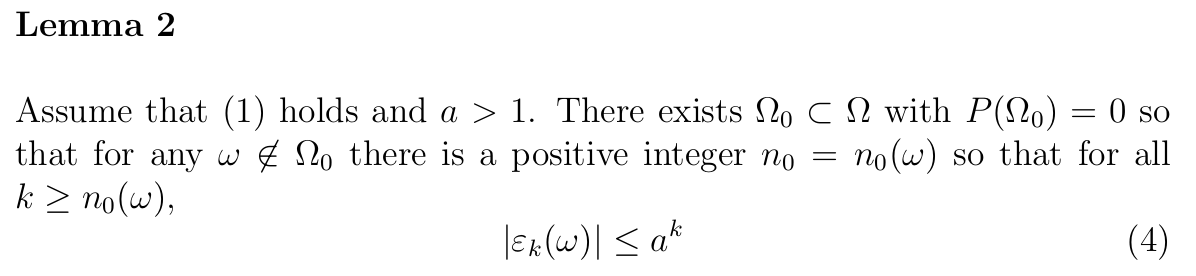
\includegraphics[width=1\linewidth]{screenshot053}
		%	\caption{}
		\label{fig:screenshot001}
	\end{figure}
	
	
	
	
	
	
\end{frame}


\section{Remark}




\begin{frame}[shrink=5]
	
	
	
	\frametitle{\insertsection} 
	\begin{figure}
		\centering
		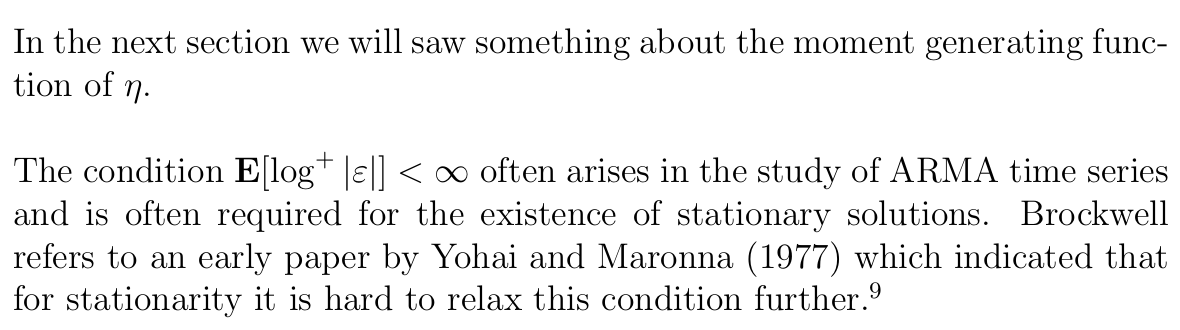
\includegraphics[width=1\linewidth]{screenshot054}
		%	\caption{}
		\label{fig:screenshot001}
	\end{figure}
	
	
	\frametitle{\insertsection} 
\begin{figure}
	\centering
	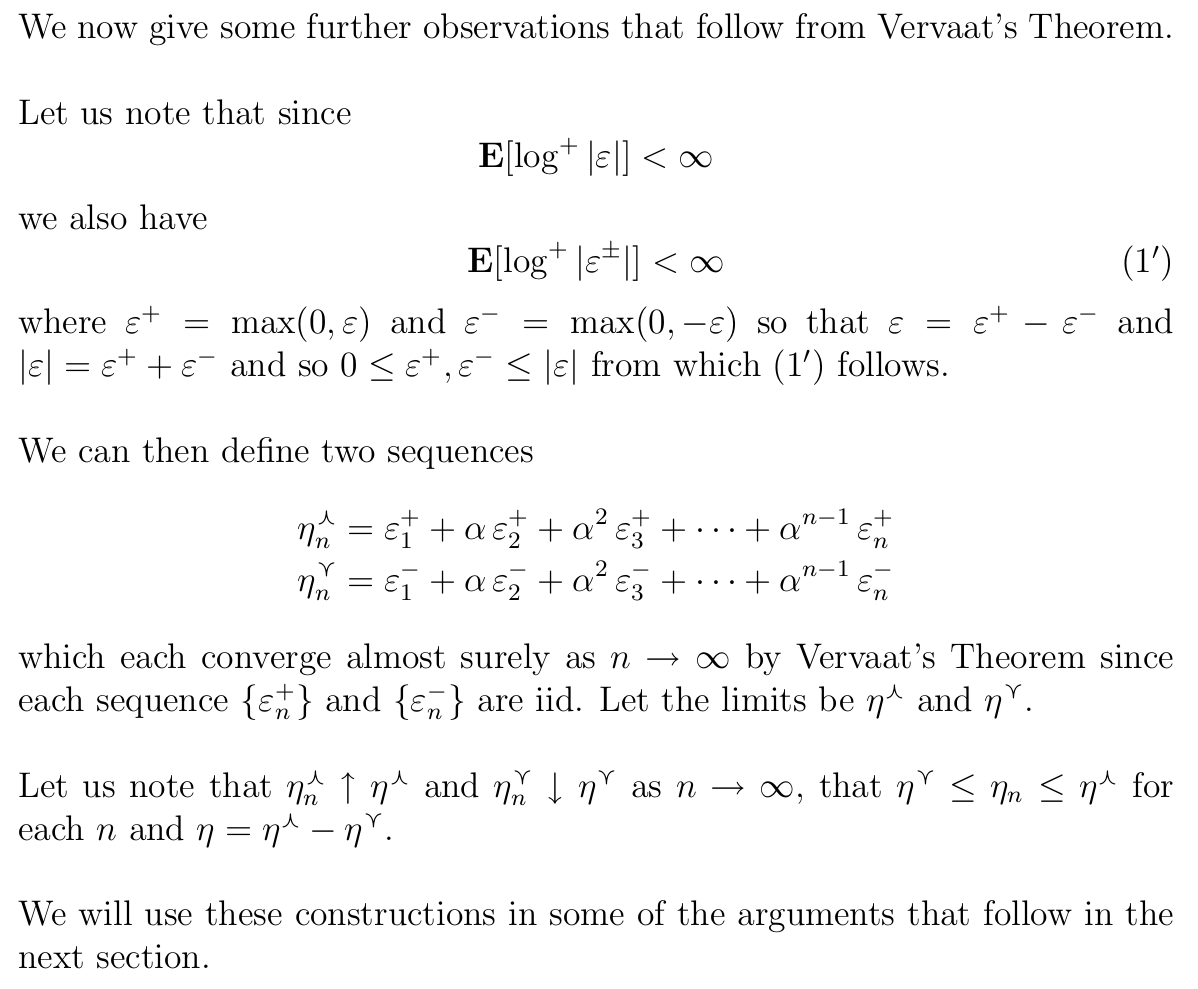
\includegraphics[width=1\linewidth]{screenshot055}
	%	\caption{}
	\label{fig:screenshot001}
\end{figure}


	
\end{frame}



\section{Contributions by Novikov}






\begin{frame}[shrink=5]
	
	
	
	\frametitle{\insertsection} 
	\begin{figure}
		\centering
		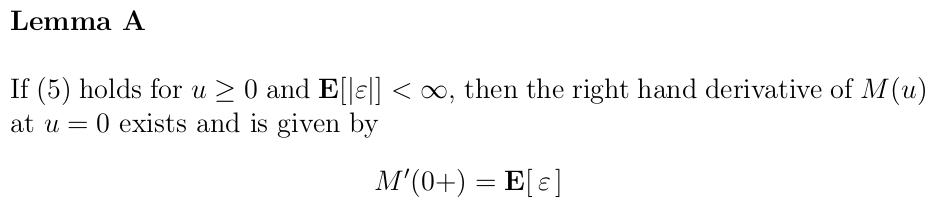
\includegraphics[width=1\linewidth]{screenshot044}
		%	\caption{}
		\label{fig:screenshot001}
	\end{figure}
	
	
		\frametitle{\insertsection} 
	\begin{figure}
		\centering
		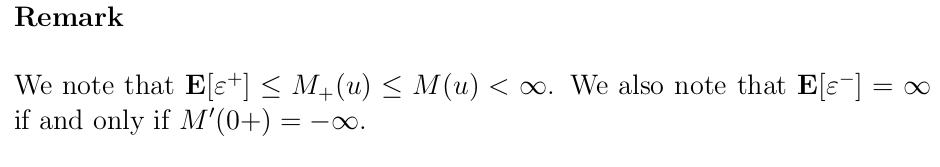
\includegraphics[width=1\linewidth]{screenshot045}
		%	\caption{}
		\label{fig:screenshot001}
	\end{figure}
	
	

	
	
\end{frame}




\begin{frame}[shrink=5]
	
	
	
	\frametitle{\insertsection} 
	\begin{figure}
		\centering
		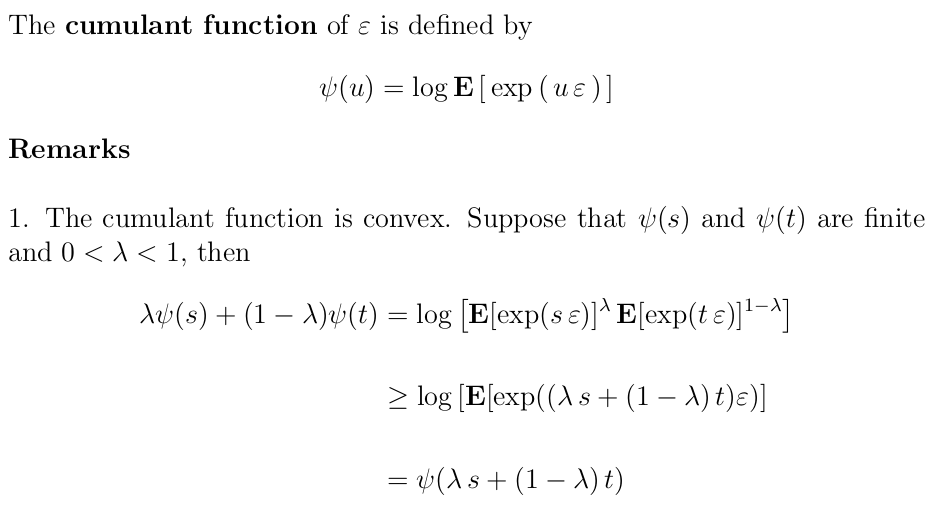
\includegraphics[width=1\linewidth]{screenshot046}
		%	\caption{}
		\label{fig:screenshot001}
	\end{figure}
	
	
	\frametitle{\insertsection} 
	\begin{figure}
		\centering
		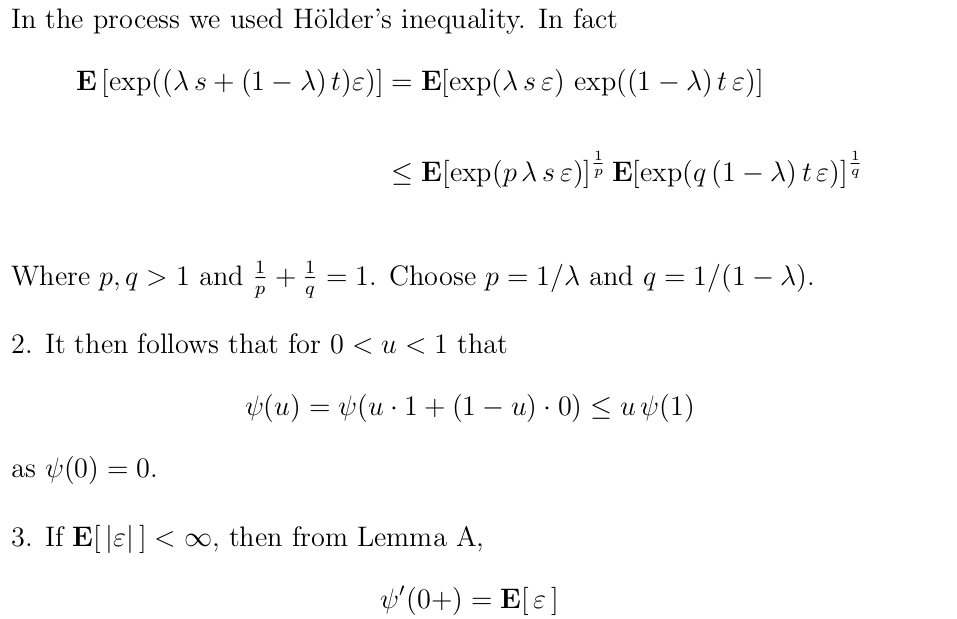
\includegraphics[width=1\linewidth]{screenshot047}
		%	\caption{}
		\label{fig:screenshot001}
	\end{figure}
	
	
	
	
	
\end{frame}

\begin{frame}[shrink=5]
	
	
	
	\frametitle{\insertsection} 
	\begin{figure}
		\centering
		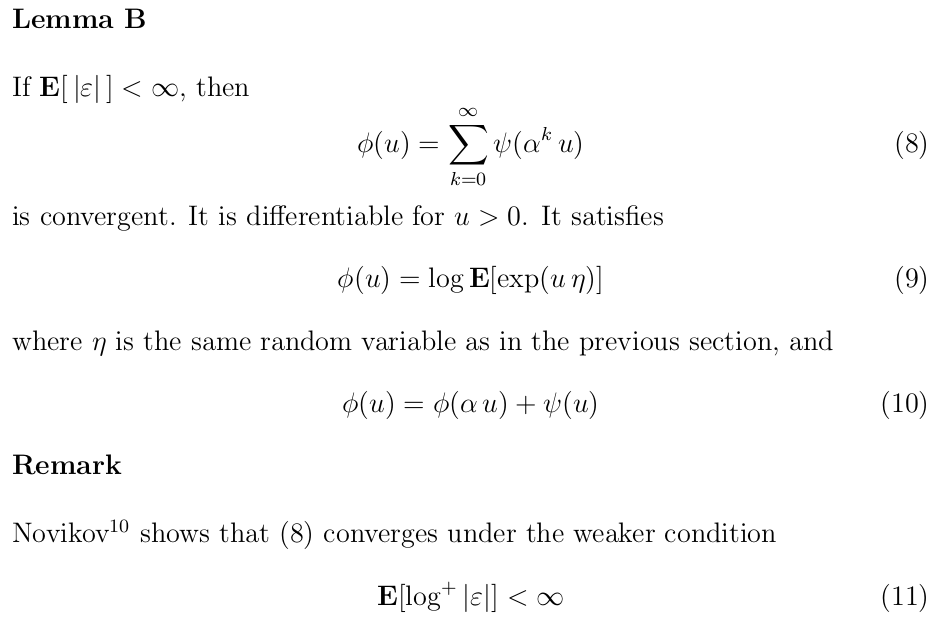
\includegraphics[width=1\linewidth]{screenshot048}
		%	\caption{}
		\label{fig:screenshot001}
	\end{figure}
	


	
	
\end{frame}

%
%\begin{frame}[shrink=5]
%	
%	
%	
%	\frametitle{\insertsection} 
%	\begin{figure}
%		\centering
%		\includegraphics[width=1\linewidth]{screenshot048}
%		%	\caption{}
%		\label{fig:screenshot001}
%	\end{figure}
%	
%	
%	
%	
%	
%\end{frame}
%

\section{Remark}


\begin{frame}[shrink=5]
	
	
	
	\frametitle{\insertsection} 
	\begin{figure}
		\centering
		\includegraphics[width=1\linewidth]{screenshot056}
		%	\caption{}
		\label{fig:screenshot001}
	\end{figure}
	
	
	
	
	
\end{frame}


\begin{frame}[shrink=5]
	
	
	
	\frametitle{\insertsection} 
	\begin{figure}
		\centering
		\includegraphics[width=1\linewidth]{screenshot057}
		%	\caption{}
		\label{fig:screenshot001}
	\end{figure}
	
	
	
	
	
\end{frame}





\end{document}	